\documentclass[12pt,a4paper]{article}

% ─── Page Layout ───────────────────────────────────────────────────────────────
\usepackage[a4paper, margin=0.8in, headheight=14pt]{geometry}

% ─── Fonts (XeLaTeX) ───────────────────────────────────────────────────────────
\usepackage{fontspec}
\usepackage{unicode-math}
\setmainfont{TeX Gyre Pagella}
\setmonofont[Scale=0.88]{TeX Gyre Cursor}
\setmathfont{Latin Modern Math}

% ─── Packages ──────────────────────────────────────────────────────────────────
\usepackage{xcolor}
\usepackage{colortbl}
\usepackage{titlesec}
\usepackage{enumitem}
\usepackage{tabularx}
\usepackage{booktabs}
\usepackage{array}
\usepackage{amsmath}
\usepackage{tikz}
\usetikzlibrary{shapes.geometric, arrows.meta, positioning, calc, fit, decorations.pathreplacing}
\usepackage{tcolorbox}
\tcbuselibrary{skins, breakable}
\usepackage{hyperref}
\usepackage{fancyhdr}
\usepackage{graphicx}
\usepackage{microtype}
\hyphenpenalty=10000
\exhyphenpenalty=10000
\sloppy
\usepackage{caption}
\usepackage{setspace}
\usepackage{multirow}
\usepackage{tocloft}

% ─── Q&A helper ────────────────────────────────────────────────────────────────
\newcommand{\Q}[1]{\textbf{#1}\par\noindent\ignorespaces}

% ─── Colour Palette ────────────────────────────────────────────────────────────
\definecolor{myred}{RGB}{196,30,58}
\definecolor{mydark}{RGB}{30,30,50}
\definecolor{mygreen}{RGB}{14,120,80}
\definecolor{myteal}{RGB}{0,130,140}
\definecolor{myamber}{RGB}{180,100,0}
\definecolor{mypurple}{RGB}{100,30,160}
\definecolor{mygray}{RGB}{246,247,249}
\definecolor{mgframe}{RGB}{180,185,200}
\definecolor{watermark}{RGB}{145,150,170}
\definecolor{hdrred}{RGB}{250,232,235}
\definecolor{hdrgreen}{RGB}{220,244,233}
\definecolor{hdrteal}{RGB}{220,242,244}
\definecolor{hdramber}{RGB}{253,242,215}
\definecolor{hdrpurple}{RGB}{238,228,255}
\definecolor{hdrgray}{RGB}{238,240,245}
\definecolor{rowalt}{RGB}{250,251,253}

% ─── Section Formatting ────────────────────────────────────────────────────────
\titleformat{\section}
  {\large\bfseries\color{myred}}{\thesection.}{0.5em}{}
  [\vspace{1pt}{\color{myred}\rule{\linewidth}{0.8pt}}]
\titleformat{\subsection}
  {\normalsize\bfseries\color{myteal}}{\thesubsection}{0.5em}{}
\titlespacing*{\section}{0pt}{18pt}{7pt}
\titlespacing*{\subsection}{0pt}{11pt}{4pt}

% ─── Paragraph ─────────────────────────────────────────────────────────────────
\setlength{\parindent}{0pt}
\setlength{\parskip}{4pt}

% ─── TOC Styling ───────────────────────────────────────────────────────────────
\renewcommand{\cfttoctitlefont}{\large\bfseries\color{myred}}
\renewcommand{\cftaftertoctitle}{\par\noindent{\color{myred}\rule{\linewidth}{0.8pt}}}
\setlength{\cftbeforetoctitleskip}{0pt}
\setlength{\cftaftertoctitleskip}{6pt}
\renewcommand{\cftsecfont}{\normalsize\bfseries\color{mydark}}
\renewcommand{\cftsecpagefont}{\normalsize\bfseries\color{mydark}}
\renewcommand{\cftsecleader}{\cftdotfill{\cftdotsep}}
\setlength{\cftbeforesecskip}{7pt}
\renewcommand{\cftsubsecfont}{\small\color{mydark}}
\renewcommand{\cftsubsecpagefont}{\small\color{mydark}}
\setlength{\cftbeforesubsecskip}{3pt}
\setlength{\cftsubsecindent}{1.4em}

% ─── Table helpers ─────────────────────────────────────────────────────────────
\renewcommand{\arraystretch}{1.45}
\setlength{\tabcolsep}{6pt}
\arrayrulecolor{mydark}
\newcolumntype{B}[1]{>{\small\bfseries\raggedright\arraybackslash}m{#1}}
\newcolumntype{Y}{>{\small\raggedright\arraybackslash}X}
\renewcommand{\tabularxcolumn}[1]{m{#1}}

% ─── Header / Footer ───────────────────────────────────────────────────────────
\pagestyle{fancy}
\fancyhf{}
\fancyhead[L]{\small\color{myred}\textbf{OE-EC604C}\;\color{mydark}--- Object Oriented Programming}
\fancyhead[R]{\small\color{myteal}\textbf{Module 6 Notes}}
\fancyfoot[C]{\small\color{mydark}\thepage}
\fancyfoot[R]{\small\color{watermark}\textit{\copyright\ Biraj}}
\renewcommand{\headrulewidth}{0.5pt}
\renewcommand{\footrulewidth}{0.3pt}

% ─── Hyperref ──────────────────────────────────────────────────────────────────
\hypersetup{
  colorlinks=true, linkcolor=myteal, urlcolor=myteal,
  pdfauthor={Biraj Sarkar},
  pdftitle={OE-EC604C --- Module 6 Notes}
}

% ─── tcolorbox styles ──────────────────────────────────────────────────────────
\tcbset{
  tikzbox/.style={
    colback=mygray, colframe=mgframe, boxrule=0.6pt, arc=4pt,
    left=8pt, right=8pt, top=6pt, bottom=6pt,
    colbacktitle=mgframe, coltitle=mydark,
    fonttitle=\small\bfseries
  },
  defbox/.style={
    colback=hdrgreen, colframe=mygreen, boxrule=0.8pt, arc=4pt,
    left=9pt, right=9pt, top=6pt, bottom=6pt,
    colbacktitle=mygreen, coltitle=white,
    fonttitle=\small\bfseries
  },
  formulabox/.style={
    colback=hdrteal, colframe=myteal, boxrule=0.8pt, arc=4pt,
    left=9pt, right=9pt, top=7pt, bottom=7pt,
    colbacktitle=myteal, coltitle=white,
    fonttitle=\small\bfseries
  },
  examplebox/.style={
    colback=hdramber, colframe=myamber, boxrule=0.8pt, arc=4pt,
    left=9pt, right=9pt, top=6pt, bottom=6pt,
    colbacktitle=myamber, coltitle=white,
    fonttitle=\small\bfseries
  },
  masonbox/.style={
    colback=hdrpurple, colframe=mypurple, boxrule=0.8pt, arc=4pt,
    left=9pt, right=9pt, top=6pt, bottom=6pt,
    colbacktitle=mypurple, coltitle=white,
    fonttitle=\small\bfseries
  },
  exambox/.style={
    colback=hdrpurple, colframe=mypurple, boxrule=1pt, arc=5pt,
    left=10pt, right=10pt, top=8pt, bottom=8pt,
    colbacktitle=mypurple, coltitle=white,
    fonttitle=\bfseries,
    breakable, title after break={\textbf{Frequently Asked / Viva Questions (contd.)}}}
}

% XeLaTeX pdfcol fix: reset text color after every tcolorbox
\tcbset{after={\color{black}}}

% ─── TikZ styles ───────────────────────────────────────────────────────────────
\tikzset{
  block/.style={rectangle, draw=myteal, fill=hdrteal,
    text width=2.4cm, align=center, minimum height=0.95cm,
    font=\small, rounded corners=3pt, line width=0.7pt},
  redblock/.style={rectangle, draw=myred, fill=hdrred,
    text width=2.4cm, align=center, minimum height=0.95cm,
    font=\small, rounded corners=3pt, line width=0.7pt},
  netnode/.style={rectangle, draw=myteal, fill=hdrteal,
    text width=1.5cm, align=center, minimum height=0.8cm,
    font=\small, rounded corners=3pt, line width=0.7pt},
  sumjunc/.style={circle, draw=myamber, fill=hdramber,
    minimum size=0.62cm, font=\small, line width=0.8pt},
  snode/.style={circle, draw=mypurple, fill=hdrpurple,
    minimum size=0.55cm, font=\footnotesize, line width=0.7pt},
  arrow/.style={-Stealth, thick, color=mydark},
  redarrow/.style={-Stealth, thick, color=myred},
  line/.style={thick, color=mydark}
}

% ═══════════════════════════════════════════════════════════════════════════════
\begin{document}
% ═══════════════════════════════════════════════════════════════════════════════

\begin{center}
  {\LARGE\bfseries\color{myred} OE-EC604C --- Object Oriented Programming}\\[5pt]
  {\normalsize\color{mydark} Semester VI \quad$\bullet$\quad 3L:0T:0P \quad$\bullet$\quad 3 Credits}\\[3pt]
  {\normalsize\color{myteal}\textbf{Module 6 Exam Notes: Inheritance}}\\[3pt]
  {\small\color{mydark} CGEC \;$|$\; B.Tech ECE (2023--27) \;$|$\; \textit{Biraj Sarkar}}
\end{center}
\vspace{2pt}
\noindent{\color{myred}\rule{\linewidth}{1.5pt}}
\vspace{2pt}

\hypersetup{linkcolor=mydark}
\tableofcontents
\hypersetup{linkcolor=myteal}
\newpage

% ===============================================================================
\section{Fundamentals of Inheritance \& Derivation Levels}
% ===============================================================================

Inheritance is the mechanism by which a new class (derived class) is built from an existing class (base class), inheriting its properties and behaviors. This promotes code reusability.

\subsection{Base and Derived Classes}
A derived class inherits members of a base class. The visibility of inherited members depends on the \textbf{inheritance access level} declared:
\begin{enumerate}[label=\textbf{\arabic*.}, leftmargin=*, itemsep=2.5pt]
  \item \textbf{Public Derivation (\texttt{class Derived : public Base}):} 
    \begin{itemize}[leftmargin=1.5em, itemsep=1pt, topsep=1pt]
      \item Public base members become \textbf{public} in the derived class.
      \item Protected base members become \textbf{protected} in the derived class.
      \item Private base members are \textbf{never accessible} directly (can only be accessed via public/protected base functions).
    \end{itemize}
  \item \textbf{Protected Derivation (\texttt{class Derived : protected Base}):} 
    \begin{itemize}[leftmargin=1.5em, itemsep=1pt, topsep=1pt]
      \item Public and protected base members become \textbf{protected} in the derived class.
    \end{itemize}
  \item \textbf{Private Derivation (\texttt{class Derived : private Base}):} 
    \begin{itemize}[leftmargin=1.5em, itemsep=1pt, topsep=1pt]
      \item Public and protected base members become \textbf{private} in the derived class.
    \end{itemize}
\end{enumerate}

\subsection{Types of Inheritance}
C++ supports five distinct inheritance topologies:
\begin{itemize}[leftmargin=*, itemsep=3pt]
  \item \textbf{Single Inheritance:} One base class, one derived class.
  \item \textbf{Multilevel Inheritance:} A class is derived from another derived class (e.g., \texttt{A -> B -> C}).
  \item \textbf{Multiple Inheritance:} A derived class has more than one base class (e.g., \texttt{A} and \texttt{B} inherited by \texttt{C}).
  \item \textbf{Hierarchical Inheritance:} Multiple derived classes inherit from a single base class.
  \item \textbf{Hybrid Inheritance:} A combination of two or more inheritance types (e.g., multiple + hierarchical).
\end{itemize}

% ===============================================================================
\section{Constructor \& Destructor Execution Sequence}
% ===============================================================================

When a derived class object is instantiated, constructors are executed along the inheritance chain to ensure that the entire object is initialized.

\subsection{Invocation Sequence Rules}
\begin{itemize}[leftmargin=*, itemsep=3pt]
  \item \textbf{Constructors:} Executed from \textbf{top to bottom} along the class hierarchy. The base class constructor is executed first, followed by the derived class constructor.
  \item \textbf{Destructors:} Executed in the \textbf{exact reverse order} (bottom to top).
  \item \textbf{Initializer Lists:} Parameterized base constructors must be explicitly called using the derived class constructor's member initialization list.
\end{itemize}

\begin{tcolorbox}[examplebox, title={Code Example: Invocation of parameterized base constructors}]
\begin{spacing}{1.0}
\begin{verbatim}
#include <iostream>
class Base {
protected:
    int baseVal;
public:
    Base(int val) : baseVal(val) {
        std::cout << "Base Constructor: " << baseVal << std::endl;
    }
    ~Base() {
        std::cout << "Base Destructor" << std::endl;
    }
};

class Derived : public Base {
private:
    int derivedVal;
public:
    // Call base constructor explicitly in initialization list
    Derived(int bVal, int dVal) : Base(bVal), derivedVal(dVal) {
        std::cout << "Derived Constructor: " << derivedVal << std::endl;
    }
    ~Derived() {
        std::cout << "Derived Destructor" << std::endl;
    }
};
\end{verbatim}
\end{spacing}
\end{tcolorbox}

% ===============================================================================
\section{The Diamond Inheritance Ambiguity}
% ===============================================================================

Multipath inheritance can result in a duplicate copy conflict known as the \textbf{Diamond Problem}.

\subsection{The Diamond Problem and Virtual Base Classes}
Consider class \texttt{D} inheriting from classes \texttt{B} and \texttt{C}, which both inherit from class \texttt{A}.
If \texttt{A} contains a member \texttt{x}, \texttt{D} receives two separate copies of \texttt{x} (one via \texttt{B} and one via \texttt{C}). Any reference to \texttt{x} inside \texttt{D} is flagged as \textbf{ambiguous} by the compiler.
\begin{tcolorbox}[defbox]
\textbf{Virtual Base Class:} By declaring the base class \texttt{A} as \texttt{virtual} during derivation in \texttt{B} and \texttt{C}, the compiler ensures that only one shared instance of class \texttt{A} is created in memory, resolving all inheritance path ambiguities.
\end{tcolorbox}

\begin{tcolorbox}[tikzbox, title={Diamond Inheritance Path Topologies}]
\centering
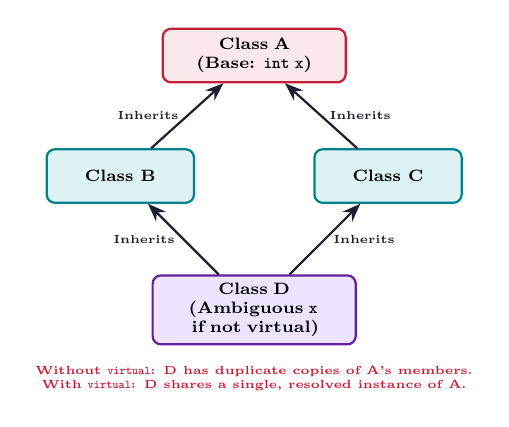
\begin{tikzpicture}[node distance=1.5cm, thick, scale=0.85, every node/.style={scale=0.85}]
  % Top Node
  \node[rectangle, draw=myred, fill=hdrred, rounded corners=3pt, align=center, text width=2.5cm, minimum height=0.8cm, font=\scriptsize\bfseries] (baseA) at (0, 1.8) {Class A \\ (Base: \texttt{int x})};

  % Middle Nodes
  \node[rectangle, draw=myteal, fill=hdrteal, rounded corners=3pt, minimum width=2.2cm, minimum height=0.8cm, font=\scriptsize\bfseries] (derB) at (-2.0, 0) {Class B};
  \node[rectangle, draw=myteal, fill=hdrteal, rounded corners=3pt, minimum width=2.2cm, minimum height=0.8cm, font=\scriptsize\bfseries] (derC) at (2.0, 0) {Class C};

  % Bottom Node
  \node[rectangle, draw=mypurple, fill=hdrpurple, rounded corners=3pt, align=center, text width=2.8cm, minimum height=1.0cm, font=\scriptsize\bfseries] (derD) at (0, -2.0) {Class D \\ (Ambiguous \texttt{x} if not virtual)};

  % Paths
  \draw[arrow] (derB) -- (baseA) node[midway, left, font=\tiny\bfseries] {Inherits};
  \draw[arrow] (derC) -- (baseA) node[midway, right, font=\tiny\bfseries] {Inherits};
  \draw[arrow] (derD) -- (derB) node[midway, left, font=\tiny\bfseries] {Inherits};
  \draw[arrow] (derD) -- (derC) node[midway, right, font=\tiny\bfseries] {Inherits};

  % Text indicators
  \node[below=0.15cm of derD, font=\tiny\bfseries\color{myred}, align=center] {Without \texttt{virtual}: D has duplicate copies of A's members.\\With \texttt{virtual}: D shares a single, resolved instance of A.};
\end{tikzpicture}
\end{tcolorbox}

\begin{tcolorbox}[examplebox, title={Code Example: Resolving Diamond Problem using Virtual Base Class}]
\begin{spacing}{1.0}
\begin{verbatim}
#include <iostream>
class A {
public:
    int x;
};

// Declare B and C with virtual public inheritance
class B : virtual public A {
public:
    int y;
};

class C : virtual public A {
public:
    int z;
};

class D : public B, public C {
public:
    int sum;
    void show() {
        x = 10; // Ambiguous without virtual keyword! Now resolved.
        y = 20;
        z = 30;
        sum = x + y + z;
        std::cout << "Sum = " << sum << std::endl;
    }
};
\end{verbatim}
\end{spacing}
\end{tcolorbox}

% ===============================================================================
\section{Containership vs. Inheritance}
% ===============================================================================

To design clean systems, software developers must choose the correct structural relationship between classes:
\begin{itemize}[leftmargin=*, itemsep=3pt]
  \item \textbf{Inheritance (\texttt{is-a} relationship):} A derived class inherits properties of the base class. E.g., a \texttt{Car} \textbf{is a} \texttt{Vehicle}.
  \item \textbf{Containership (\texttt{has-a} relationship):} An object of one class is embedded as a data member inside another class. E.g., a \texttt{Car} \textbf{has an} \texttt{Engine}.
\end{itemize}

% ===============================================================================
% MANDATORY QUICK REVISION PAGE
% ===============================================================================
\newpage
\begin{center}
  {\large\bfseries\color{myred} Quick Revision --- Module VI}\\[3pt]
  {\small\color{mydark} Inheritance $|$ OE-EC604C}
\end{center}
\noindent{\color{myred}\rule{\linewidth}{1.2pt}}
\vspace{4pt}

\begin{tcolorbox}[formulabox, title={\textbf{Access Control Table under Derivation}}]
\renewcommand{\arraystretch}{1.3}
\par\noindent
\begin{tabularx}{\linewidth}{|B{2.8cm}|Y|Y|Y|}
\hline
\textbf{Base Member} & \textbf{Public Derivation} & \textbf{Protected Derivation} & \textbf{Private Derivation} \\
\hline
\textbf{Private}     & Not Accessible & Not Accessible & Not Accessible \\
\hline
\textbf{Protected}   & Protected in Derived & Protected in Derived & Private in Derived \\
\hline
\textbf{Public}      & Public in Derived & Protected in Derived & Private in Derived \\
\hline
\end{tabularx}
\end{tcolorbox}

\begin{tcolorbox}[defbox, title={\textbf{One-Line Definitions}}]
\begin{itemize}[leftmargin=*, itemsep=2.5pt, topsep=0pt]
  \item \textbf{Inheritance:} The mechanism of deriving a new class from an existing base class to reuse code.
  \item \textbf{Base Class:} The existing class from which features are inherited.
  \item \textbf{Derived Class:} The new class that inherits features from one or more base classes.
  \item \textbf{Diamond Problem:} An ambiguity issue where a derived class inherits duplicate members of a grandparent class through two distinct paths.
  \item \textbf{Virtual Base Class:} A base class declared virtual to ensure only one instance is shared in multipath inheritance.
  \item \textbf{Containership:} Embedding an object of one class as a member variable inside another class (Composition).
  \item \textbf{Initialization List (Base):} The derived constructor syntax used to pass arguments to base class constructors.
  \item \textbf{Is-A Relationship:} Logical relationship modeled by class inheritance (e.g., Dog is-a Mammal).
  \item \textbf{Has-A Relationship:} Logical relationship modeled by class containership (e.g., Dog has-a Tail).
\end{itemize}
\end{tcolorbox}

\begin{tcolorbox}[exambox, title={\textbf{Frequently Asked / Viva Questions}}]
\begin{enumerate}[topsep=0pt, label=\textbf{Q\arabic*.}, itemsep=5pt]
  \item \Q{Why are private base class members not accessible in derived classes?}
    This maintains the privacy boundaries of class design. If derived classes could access private members directly, encapsulation could be easily broken.
  \item \Q{Explain why virtual inheritance is necessary to solve the Diamond Problem.}
    Virtual inheritance directs the compiler to build only one shared instance of the grandparent class, resolving lookup ambiguity for its members.
  \item \Q{What is the execution order of constructors in multiple inheritance?}
    Base constructors are executed in the order they are listed in the inheritance declaration, NOT the order they appear in the initializer list. E.g., \texttt{class D : public B, public C} calls B's constructor first, then C's.
  \item \Q{Which class constructor is executed first in multilevel inheritance?}
    The absolute root base class constructor is executed first, followed by intermediate bases, ending at the leaf derived class.
  \item \Q{Does a derived class inherit the constructor of the base class?}
    No. Constructors are class-specific and are not inherited. A derived class must define its own constructors or use the default constructor.
  \item \Q{Can we declare a destructor virtual? Why?}
    Yes, virtual destructors are mandatory when deleting derived objects via base pointers to ensure derived resource cleanup.
  \item \Q{What is the difference between multiple inheritance and hybrid inheritance?}
    Multiple inheritance involves deriving from 2+ distinct base classes. Hybrid inheritance combines multiple topologic models (like multiple and multilevel).
  \item \Q{How does containership differ from private inheritance?}
    Containership embeds objects as members, restricting them to public APIs. Private inheritance makes base members private, permitting code access but hiding public APIs from external callers.
  \item \Q{What happens if base and derived classes declare members with the same name?}
    The derived member hides the base member. The base member can still be accessed using the scope resolution operator: \texttt{BaseClass::memberName}.
  \item \Q{Can a class inherit from itself in C++?}
    No, circular or self-inheritance (e.g., \texttt{class A : public A}) is syntactically invalid and causes compile errors.
  \item \Q{Why does virtual inheritance require base class constructors to be called by the most derived class?}
    Since the base class instance is shared, intermediate derived classes cannot initialize it independently. The most derived class constructor executes its initialization.
  \item \Q{How does the visibility level of inheritance affect derived class inheritance hierarchies?}
    Private inheritance prevents downstream subclasses from accessing grandparent class members, whereas public/protected inheritances allow subclass access.
\end{enumerate}
\end{tcolorbox}

\begin{tcolorbox}[tikzbox, title={Comparison: Multiple Inheritance vs. Hybrid Inheritance}]
\renewcommand{\arraystretch}{1.45}
\par\noindent
\begin{tabularx}{\linewidth}{|B{3.2cm}|Y|Y|}
\hline
\textbf{Feature} & \textbf{\color{myteal}Multiple Inheritance} & \textbf{\color{myamber}Hybrid Inheritance} \\
\hline
\textbf{Structure} & A single subclass derives directly from two or more parent classes. & Combines two or more basic inheritance shapes (e.g., hierarchic, multilevel, multiple). \\
\hline
\textbf{Diamond Risk} & None, unless parent classes share a common grandparent class. & High. Multipath inheritance frequently creates diamond path ambiguities. \\
\hline
\textbf{Complexity} & Moderate. Simple to resolve using qualifiers. & High. Requires virtual inheritance declaration to resolve duplicate members. \\
\hline
\textbf{Design Goal} & Merging features from multiple independent source interfaces. & Modeling complex real-world classification hierarchies. \\
\hline
\end{tabularx}
\end{tcolorbox}

\end{document}
